\documentclass[conference]{IEEEtran}
\usepackage{amsmath,amssymb,booktabs,graphicx,url}
\usepackage[hidelinks]{hyperref}
\usepackage{tikz}
\usetikzlibrary{arrows.meta,positioning}
\graphicspath{{../figures/}}
\title{Cross-Institution Reliability of Temporal Attributions in Network Traffic Forecasting}
\author{\IEEEauthorblockN{Anonymous research draft}\IEEEauthorblockA{Conference draft; authors and venue to be finalized}}
\begin{document}\maketitle
\begin{abstract}
Forecast accuracy does not establish that temporal explanations remain useful at unseen institutions. We audit this distinction on CESNET-TimeSeries26 using 32 source institutions, eight validation institutions and two target cohorts: eight original targets and 32 subsequently reserved targets. The latter cohort reuses the locked source models, yielding 80 unique institutions within one ISP. Ridge, DLinear and GRU predict one- and six-hour endpoints from one week of history. We separate forecast error, numerical attribution checks and ranking alignment under controlled history replacements. The original primary target-minus-source Shapley contrast for frozen one-hour GRU is $-0.0189$, nominal 95\% interval $[-0.0891,0.0533]$, across seven complete pairs. The new-cohort contrast is $-0.0075$, interval $[-0.0402,0.0241]$, across 30 pairs; a prespecified denser timestamp budget also spans zero. Neither establishes degradation or equivalence. Original reference-specific secondary intervals below zero do not recur in the new cohort. Extreme relative forecast errors on nearly constant traffic and undefined ranking games further limit complete-case inference. The contribution is a reproducible empirical reliability audit with explicit references, numerical failures and effective denominators.
\end{abstract}
\begin{IEEEkeywords}network traffic forecasting, explainability, institution transfer, temporal attribution, evaluation\end{IEEEkeywords}

\section{Introduction}
Network traffic forecasting supports resource planning, but prediction and explanation require different evidence. Forecast error compares a prediction with a future observation. Temporal attribution allocates a prediction contrast over historical inputs. A ranking test measures response to a specified replacement of those inputs. Accuracy, an attribution identity and ranking alignment therefore cannot certify one another. This distinction matters when a pooled forecaster serves an institution absent from fitting.

Transfer forecasting~\cite{transmuse}, network forecasting explanations~\cite{aichrono} and explanation generalization under shift~\cite{timesae} are established research. Our question is narrower: under an institution-disjoint network deployment protocol, what evidence supports the reliability of temporal attribution rankings, and how does that evidence depend on references, operators and score availability?

We study public institutional traffic~\cite{cesnet26,dataset} with source-only fitting, unseen validation institutions, timestamp-matched source/target cases and a fixed primary contrast. After the original eight-target result, we freeze an additional 32-target cohort before scoring it. Sources and models remain shared, so the estimates are reported separately. Our contributions are (i) an executed deployment benchmark separating accuracy, numerical validity and operator-response alignment; (ii) explicit attribution references, exclusion denominators and paired uncertainty; and (iii) a new-target within-network replication with prespecified sampling-density and uncertainty sensitivities. We contribute empirical evidence and controls, rather than a new attribution algorithm.

Both primary intervals contain zero. The stronger-looking original secondary pattern under a history-median reference does not recur as an interval excluding zero in the larger cohort. We retain these outcomes and the excluded low-volume regimes. Figure~\ref{fig:pipeline} gives the complete workflow; supplementary material preserves the extended diagnostics and reproduction details.

\begin{figure*}[t]\centering
\resizebox{\textwidth}{!}{% Compact editable workflow; orthogonal connectors, no raster scaling.
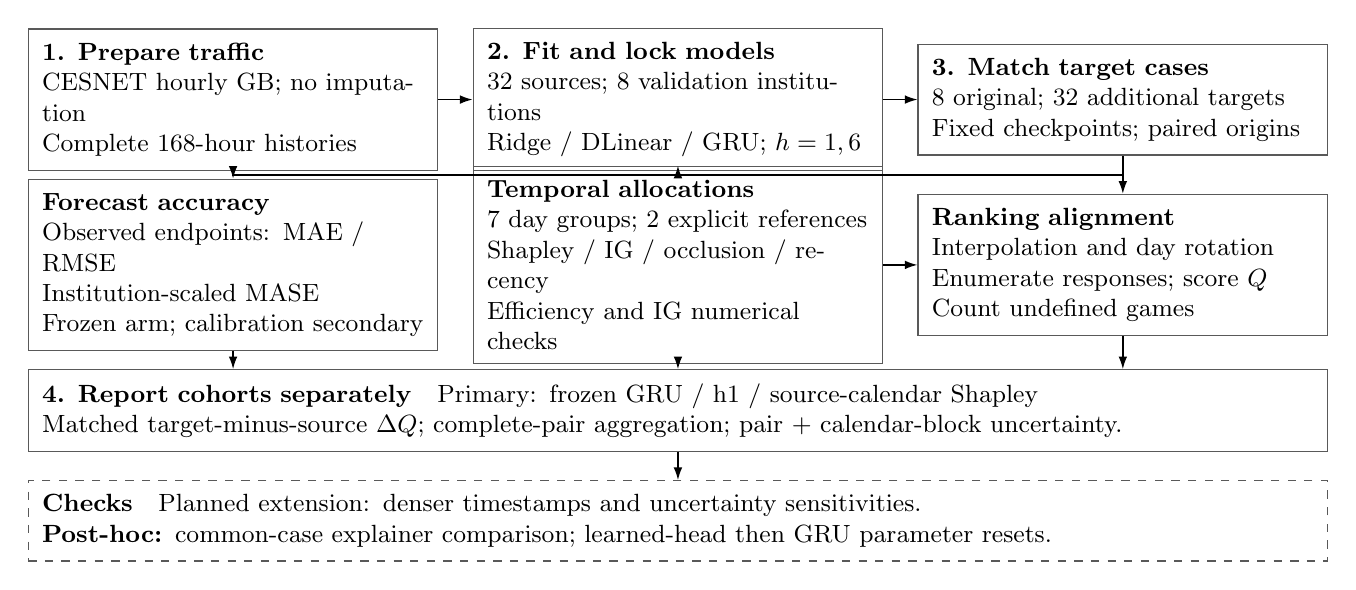
\begin{tikzpicture}[
 x=1cm,y=1cm,font=\small,
 block/.style={draw=black!65,line width=.45pt,align=left,inner sep=5pt},
 col/.style={block,text width=4.85cm,minimum height=1.35cm},
 wide/.style={block,text width=16.15cm},
 flow/.style={-{Latex[length=1.6mm,width=1.1mm]},line width=.5pt}
]
\node[col] (data) at (-5.65,0)
{\textbf{1. Prepare traffic}\\CESNET hourly GB; no imputation\\Complete 168-hour histories};
\node[col] (fit) at (0,0)
{\textbf{2. Fit and lock models}\\32 sources; 8 validation institutions\\Ridge / DLinear / GRU; $h=1,6$};
\node[col] (cases) at (5.65,0)
{\textbf{3. Match target cases}\\8 original; 32 additional targets\\Fixed checkpoints; paired origins};
\draw[flow] (data.east)--(fit.west);
\draw[flow] (fit.east)--(cases.west);

\node[col,minimum height=1.75cm] (accuracy) at (-5.65,-2.1)
{\textbf{Forecast accuracy}\\Observed endpoints: MAE / RMSE\\Institution-scaled MASE\\Frozen arm; calibration secondary};
\node[col,minimum height=1.75cm] (attr) at (0,-2.1)
{\textbf{Temporal allocations}\\7 day groups; 2 explicit references\\Shapley / IG / occlusion / recency\\Efficiency and IG numerical checks};
\node[col,minimum height=1.75cm] (response) at (5.65,-2.1)
{\textbf{Ranking alignment}\\Interpolation and day rotation\\Enumerate responses; score $Q$\\Count undefined games};
\draw[flow] (cases.south)--(5.65,-.96)--(-5.65,-.96)--(accuracy.north);
\draw[flow] (0,-.96)--(attr.north);
\draw[flow] (5.65,-.96)--(response.north);
\draw[flow] (attr.east)--(response.west);

\node[wide,minimum height=.9cm] (report) at (0,-3.95)
{\textbf{4. Report cohorts separately}\quad Primary: frozen GRU / h1 / source-calendar Shapley\\Matched target-minus-source $\Delta Q$; complete-pair aggregation; pair + calendar-block uncertainty.};
\draw[flow] (accuracy.south)--(report.north -| accuracy.south);
\draw[flow] (attr.south)--(report.north);
\draw[flow] (response.south)--(report.north -| response.south);

\node[wide,dashed,minimum height=.85cm] (checks) at (0,-5.35)
{\textbf{Checks}\quad Planned extension: denser timestamps and uncertainty sensitivities.\\\textbf{Post-hoc:} common-case explainer comparison; learned-head then GRU parameter resets.};
\draw[flow] (report.south)--(checks.north);
\end{tikzpicture}
}
\caption{Executed workflow and separately frozen extension. Source fitting, validation, both deployment arms, attribution references, numerical screening, independent replacement definitions and paired inference remain distinct. Hash freezes are local audit trails; controlled responses do not identify causal demand effects.}\label{fig:pipeline}
\end{figure*}

\section{Related Work}
TransMUSE~\cite{transmuse} studies transferable network forecasting. DLinear~\cite{dlinear}, GRU~\cite{gru}, CESNET forecasting comparisons~\cite{comparison} and the dataset descriptor~\cite{cesnet26} motivate compact baselines and evaluation across institutions and years. AIChronoLens~\cite{aichrono} connects explanations with mobile-network temporal properties and forecast errors. Aggregated network explanations~\cite{aggregated} and attacks on forecasting explainability~\cite{deexp} address other aspects of reliability. Our study isolates unseen-institution deployment on byte-volume series.

IG explains a path-dependent contrast~\cite{ig}; Shapley attribution allocates a coalition game~\cite{shap}. Reference choice changes the explained question~\cite{manyshap,baselines}, and an efficiency identity alone does not validate its meaning. Sanity checks~\cite{sanity}, learned perturbations~\cite{perturb} and InterpretTime~\cite{interprettime} motivate auditing evaluation procedures. TIMING~\cite{timing} already addresses signed temporal effects and cumulative responses; cancellation awareness is not our novelty. TimeSAE~\cite{timesae} already examines explanation generalization under shift. Our bounded contribution combines institutional deployment controls with numerical and ranking audits on observed network traffic. We do not benchmark or claim superiority over these specialized explainers.

\section{Data and Deployment Protocol}
\subsection{Cohorts, chronology and eligibility}
We use official hourly institutional \texttt{n\_bytes} from CESNET-TimeSeries26, Zenodo record 21945629, under CC BY 4.0~\cite{dataset}. All institutions belong to the CESNET3 ecosystem~\cite{cesnet26}; they are not independent ISPs. Archive checksums, source-member hashes and derived-file hashes are recorded. Values become decimal GB ($10^9$ bytes); no classification labels or synthetic traffic mixtures enter the benchmark.

A usable hour has six native ten-minute records and an observed finite nonnegative value. Every input requires 168 usable hourly values and observed endpoints at $h=1,6$. Zeros remain observed zeros; missing values are not imputed. A conservative global flag excludes windows crossing 21 May--4 June 2024 because of a documented probe-artifact concern whose institution-specific extent is uncertain.

Twelve earlier development institutions are excluded. Deterministic SHA-256 ordering within four 2024 median-volume strata selects the original 32 sources, eight validation institutions and eight targets. Eight source--target pairs are matched within strata using 2024 median volume and coefficient of variation. Matching is descriptive, not causal identification. Source training targets are in 2024; validation uses January--March 2025. Evaluation endpoints lie in [8 April, 1 July) in 2025 and 2026, with origins at UTC hours divisible by six.

The additional cohort excludes all 48 original institutions and the 12 development institutions. Among 217 eligible unused candidates, a fixed hash salt selects eight per reconstructed volume stratum. Hungarian matching within strata pairs these 32 new targets with all 32 original source anchors using source-standardized log-transformed 2024 median volume and coefficient of variation. There is no outcome-based caliper or replacement. The original outcome was already known when this protocol was written; new membership and then code/data/timestamps were locally frozen before new-target scoring. This is not external preregistration or independent network replication. Both studies together contain 80 unique institutions.

\begin{table}[t]\centering
\caption{Effective evaluation units. Histories and repeated queries do not increase the number of institutions.}\label{tab:units}
\begin{tabular}{lrr}\toprule
Quantity&Original&New targets\\\midrule
Target institutions&8&32\\
Matched source anchors&8&32\\
Available matched pair-years&15/16&63/64\\
Target forecast institution-year cells&15&63\\
Main XAI histories per fitted model&480&2,016\\
IG histories per fitted model&120&504\\
Complete primary pairs&7&30\\
Dense GRU histories per seed&---&8,064\\\bottomrule
\end{tabular}\end{table}

For explanations, intersect eligible timestamps per matched pair/year and choose up to 16 evenly spaced origins using availability only; four form the IG subset. Original pair 2 (source 160, target 192) lacks a common 2026 cell. New pair 1 (source 260, target 8) also lacks one; neither is replaced. Original 2026 target cells have only 50 or 129 eligible origins versus 206 or 307 in 2025. Complete-case conclusions concern observed eligible regimes, not interrupted or absent periods. Table~\ref{tab:units} separates sampling budgets from inferential units.

\subsection{Locked predictors and accuracy metrics}
Inputs use $\log(1+x)$; two heads predict endpoints directly. The deployed GB function, including clipping, is
\begin{equation}
F_h(x)=\exp\!\left(\max\{0,z_h(\log(1+x))\}\right)-1.
\end{equation}
Ridge fits separate horizon heads; validation selects $\alpha=0.1$ from $\{0.1,1,10,100\}$. DLinear uses a 25-hour moving-average decomposition and two 168-to-2 linear maps (676 parameters). GRU uses one 32-unit layer and a correction to the last log input (3,426 parameters). Persistence, daily and weekly seasonal forecasts are comparators.

Neural fitting uses source-only scalar normalization, Adam, batch size 256, log-space MSE and gradient clipping at one. There are 227,478 eligible overlapping source-training windows; each epoch samples 1,024 per source, or 32,768. Training permits 30 epochs with patience five. Seed 42 chooses between learning rates $10^{-3}$ and $3\cdot10^{-4}$; seeds 123 and 2026 reuse the choice. Selected rates are $3\cdot10^{-4}$ for DLinear and $10^{-3}$ for GRU. New targets never enter fitting or tuning; the replication preserves checkpoint bytes and source references.

Accuracy uses MAE/RMSE in GB and MASE with each institution's eligible 2024 weekly absolute-difference scale, floored at $10^{-9}$ GB. We average neural seeds first, then available institution-year cells; unequal availability can change weighting. Prespecified supplementary summaries also average years within institution first and report years separately. A secondary calibrated arm adds a local median log-residual offset from 1--8 April, with at least 24 eligible examples; otherwise it uses zero and flags the case. This arm uses local observations; frozen models define the primary endpoint.

\section{Attribution and Ranking Measurements}
\subsection{Reference-explicit allocations and numerical checks}
Seven consecutive 24-hour groups run from oldest to newest. The source-calendar reference is the source-2024 pooled median by hour of week. The history-hour-median reference repeats the current history's median for each hour of day. Neither uses future endpoints.

For reference $r$, input $x$ and groups $N$, the retained-group game is $v(S)=F(x_S,r_{\bar S})$. All $2^7=128$ coalitions give exact Shapley values
\begin{equation}
\phi_j=\sum_{S\subseteq N\setminus\{j\}}\frac{|S|!(6-|S|)!}{7!}\big[v(S\cup\{j\})-v(S)\big].
\end{equation}
We check $\sum_j\phi_j=F(x)-F(r)$ in double precision. Occlusion ranks the absolute single-group replacement effect; recency ranks newest first. Shapley and IG rank the absolute signed daily sum, so opposing hourly effects can cancel within a group.

IG integrates raw-GB gradients along the straight reference-to-input path~\cite{ig}, using 32, 64, 128, 256 and at most 512 Gauss--Legendre nodes. Acceptance requires both completeness error and successive L1 refinement change below $10^{-8}$ GB plus $10^{-3}$ times the absolute prediction contrast or L1 attribution, respectively. Rejected cases remain recorded and receive no IG ranking score. Numerical acceptance does not establish on-manifold paths, correct demand causes or useful rankings.

\subsection{Controlled ranking-response game}
Two replacement templates are distinct from attribution references: within-day straight-line interpolation between observed endpoints, and cyclic one-day rotation of the observed week. They suppress variation or exchange day blocks without future labels, but need not be natural traffic draws. Their log-input RMS displacement is retained.

For order $\pi$, let $x^{(j)}$ replace its first $j$ groups. Define
\begin{align}
C_k(\pi)&=\sum_{j=1}^{k}|F(x^{(j)})-F(x^{(j-1)})|,\\
U(\pi)&=\tfrac13\{C_1(\pi)+C_2(\pi)+C_4(\pi)\},\\
Q(\pi)&=\frac{U(\pi)-R}{O-R}.
\end{align}
All $7!=5,040$ orders are enumerated from cached replacement-coalition responses: $R$ is their exact mean utility and $O$ their maximum. Cumulative response relates to cancellation-aware evaluation~\cite{timing}. $Q$ is undefined when $O-R\leq10^{-9}$ GB; otherwise zero denotes random-order mean and one the operator response oracle. Negative scores are allowed. The oracle optimizes model response, not forecast accuracy or operational demand utility. Large responses can reflect brittleness.

\subsection{Primary inference and fixed sensitivities}
The primary contrast is target-minus-source $Q$ for frozen GRU, h1 and source-calendar Shapley. Require all three seeds to be defined before averaging; pair source and target at the same origin/operator. Average within pair/year/operator, equally over both years and operators, then equally over complete pairs. Seeds and queries are not independent institutions.

The original uncertainty procedure attempts 2,000 pair/within-pair 14-day-block bootstrap draws. Source, target and operator rows travel together; draws missing an operator cell are invalid. A nominal percentile 95\% interval requires at least four complete pairs and 1,000 valid draws. The new cohort retains this primary procedure. Other models, references, horizons, calibration and IG comparisons are secondary, without multiplicity correction.

Before new-target scoring we also fixed pair-only cluster resampling, conditional on observed periods, and synchronized calendar resampling: six 14-day block labels per year shared across sampled pairs. Both attempt 2,000 draws, with the same valid-draw gate for synchronized blocks. A nested dense budget retains the main origins and adds up to 48 per pair/year. It evaluates frozen GRU seeds at both horizons with source-calendar Shapley/occlusion/recency, without dense IG or calibration. Own-panel and common-complete-pair comparisons are both reported; a sensitivity is not promoted to primary after its outcome.

\section{Results}
\subsection{Primary transfer contrasts and replication}
Original source and target mean $Q$ are 0.7006 and 0.6817 across seven complete pairs: $\Delta Q=-0.0189$, nominal interval $[-0.0891,0.0533]$, 1,853/2,000 valid draws. The new-cohort primary is $-0.0075$, interval $[-0.0402,0.0241]$, 30 complete pairs, 1,885 valid draws. Figure~\ref{fig:uncertainty} reports them separately with every prespecified new-cohort uncertainty family. None establishes systematic degradation or equivalence; no equivalence/non-inferiority margin was specified.

\begin{figure*}[t]\centering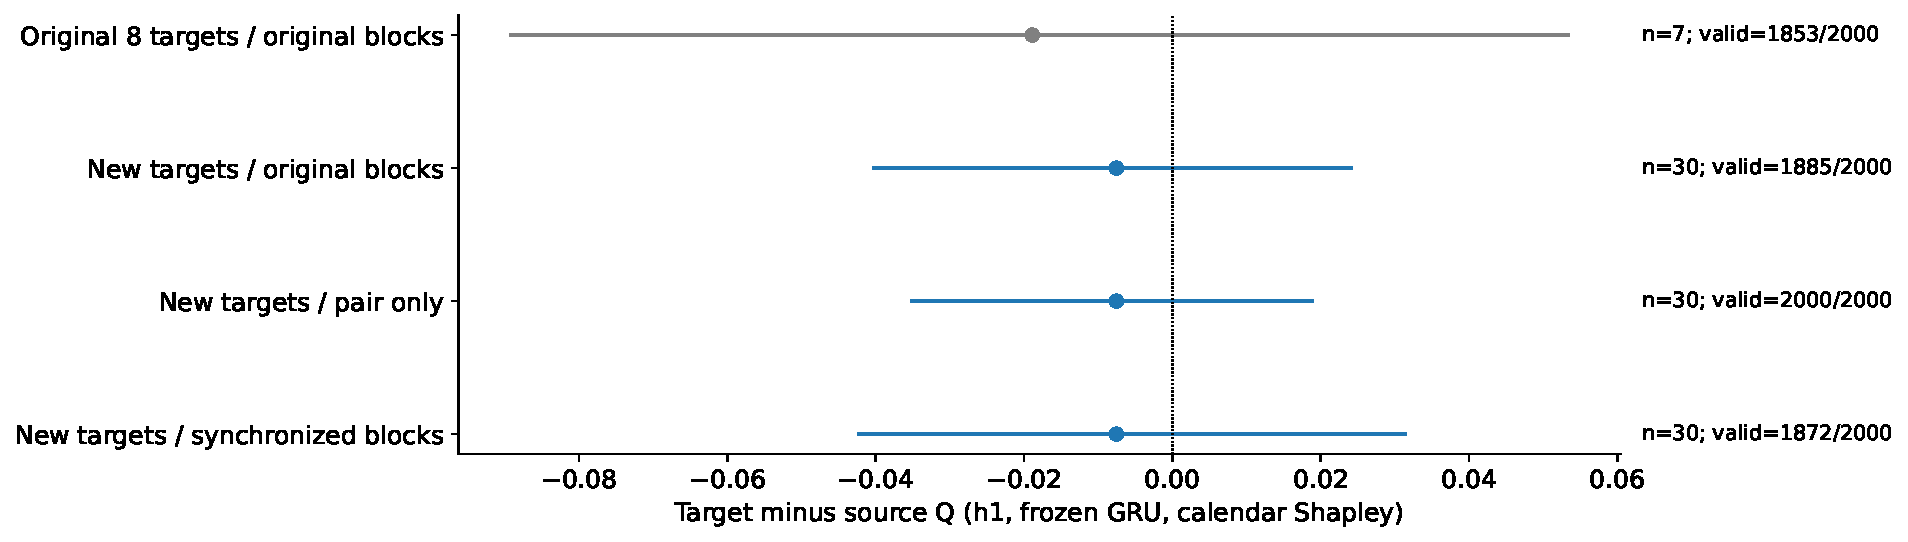
\includegraphics[width=.96\textwidth]{replication_uncertainty.pdf}
\caption{Separate original/new h1 contrasts and prespecified new-cohort uncertainty sensitivities. Pair-only intervals condition on observed periods. Sources, models and ISP overlap; these are not independent network replications. All displayed nominal intervals include zero.}\label{fig:uncertainty}
\end{figure*}

New pair-only resampling gives $[-0.0350,0.0188]$ (2,000 valid draws); synchronized calendar blocks give $[-0.0422,0.0313]$ (1,872 valid). Dense h1 is $+0.0001$, interval $[-0.0229,0.0248]$ (2,000 valid), while dense h6 is $-0.0197$, interval $[-0.0534,0.0090]$ (1,988 valid). Main h6 is $-0.0034$, interval $[-0.0417,0.0314]$. All main/dense comparisons retain the same 30 complete pairs, so point changes here do not come from different pair membership (Fig.~\ref{fig:density}).

\begin{figure*}[t]\centering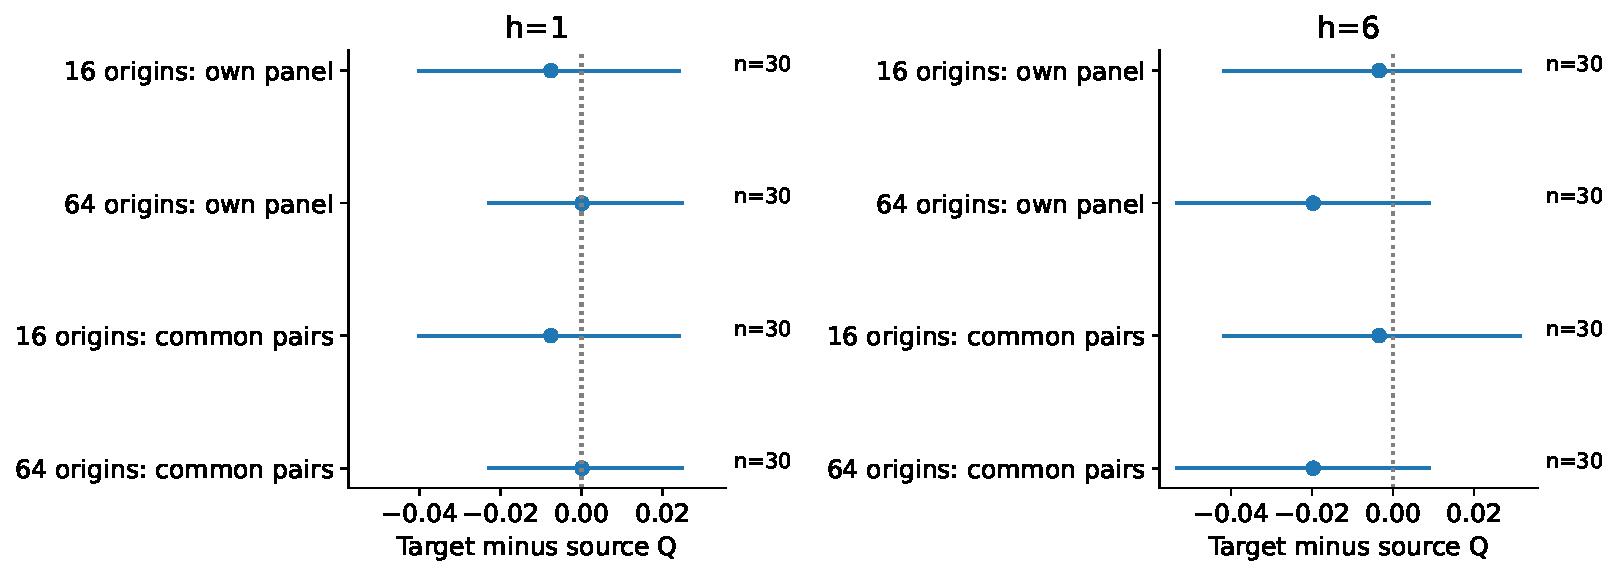
\includegraphics[width=\textwidth]{replication_density.pdf}
\caption{Prespecified 16-to-64-origin sensitivity, using original pair/within-pair block intervals. Own and common-complete-pair panels coincide here (30 pairs). Main cases are reused exactly; added cases are queried separately.}\label{fig:density}
\end{figure*}

The original h1 history-median secondary intervals fall below zero for all three forecasters; all twelve fixed new-cohort model/horizon/reference Shapley intervals include zero. This does not formally test a cohort difference, but the original reference-specific zero-excluding pattern does not recur. The supplementary material retains the original secondary forest, operator components and post-hoc leave-one-pair-out diagnostic.

\subsection{Accuracy and low-volume failures}
Table~\ref{tab:forecast} shows frozen target MASE, retaining each original scale and every available institution-year. The original one-hour model means are close; the larger cohort exposes extreme relative errors that the smaller target set missed. DLinear's lower descriptive mean does not establish inferential superiority.

\begin{table}[t]\centering
\caption{Frozen target mean MASE. Average seeds before available institution-year cells (15 original, 63 new). No case removal or significance ranking.}\label{tab:forecast}
\begin{tabular}{lrrrr}\toprule
&\multicolumn{2}{c}{Original targets}&\multicolumn{2}{c}{New targets}\\
Model&h1&h6&h1&h6\\\midrule
Persistence&0.737&1.451&1.408&2.428\\
Daily&1.083&1.112&1.864&1.824\\
Weekly&1.075&1.053&1.673&1.674\\
Ridge&0.681&0.813&30.823&57.324\\
DLinear&0.682&0.812&1.208&1.375\\
GRU&0.684&0.909&9.682&64.150\\\bottomrule
\end{tabular}\end{table}

After observing extreme new-cohort MASE, we added a descriptive all-cell scale diagnostic (Fig.~\ref{fig:scales}), retaining the metric, floor and membership. Target 267 has a 2024 weekly scale of about 751 bytes. GRU seed 2026 h6 yields approximately 0.004445 GB MAE in 2025, hence MASE about 5,921. Small absolute errors can dominate a mean of relative ratios. Descriptive h1 median institution-year MASE is 0.761 for Ridge, 0.747 for DLinear and 0.824 for GRU; medians do not replace the frozen means.

\begin{figure*}[t]\centering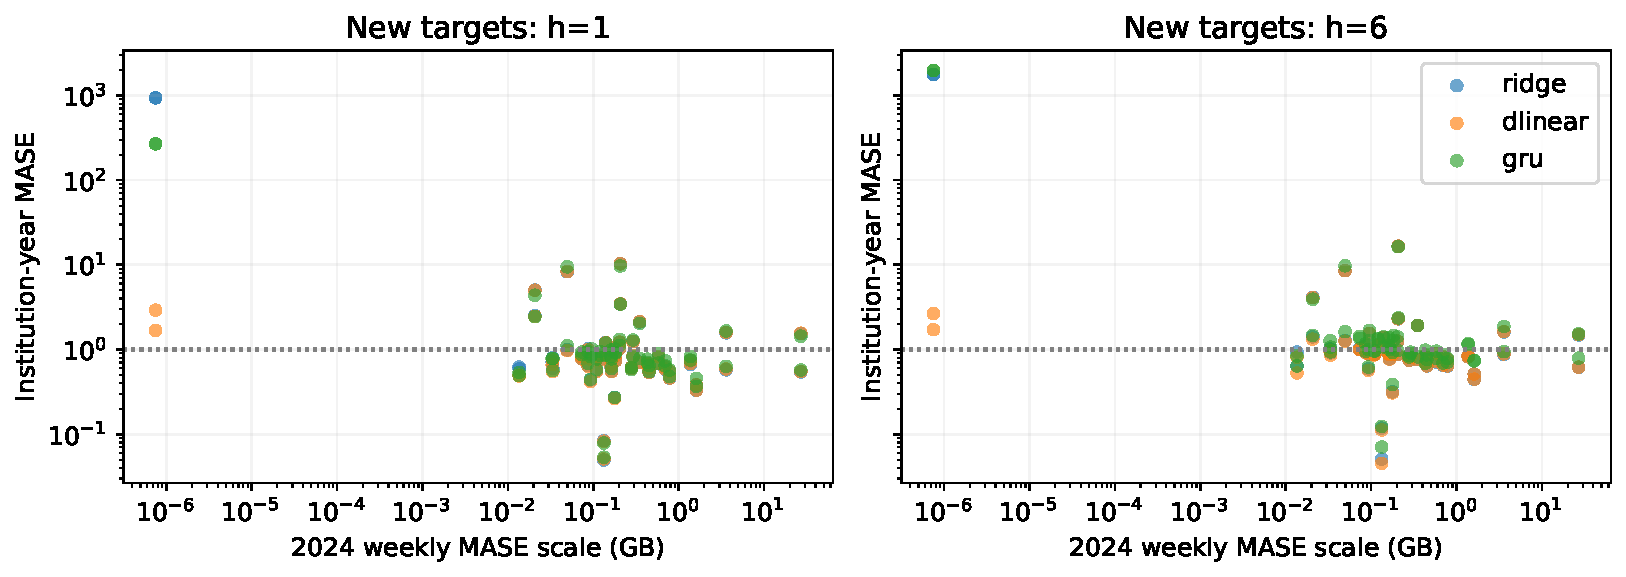
\includegraphics[width=\textwidth]{replication_forecast_scales.pdf}
\caption{Post-hoc forecast-scale diagnostic retaining all new-target institution-year cells. Both axes are logarithmic. Nearly constant low-volume series can have extreme relative errors; no metric capping, floor change or case exclusion is applied.}\label{fig:scales}
\end{figure*}

\subsection{Attribution validity and effective denominators}
The original numerical audit rejects 210/3,360 IG checks; the new main audit rejects 690/14,112. These are numerical cases across references, horizons and seeds, not independent subjects. Original Shapley efficiency residuals are at most $3.56\cdot10^{-15}$ GB; independent permutation enumeration agrees with subset arithmetic on audited cases. Failed IG cases never receive ranking scores.

In the original study, 51,944/53,760 operator-score records are defined for each non-IG method; accepted/defined IG has 6,137/6,720 records. The new audit retains 705,600 ranking records, including undefined values. New pair 4 (source 281, target 267) has no complete three-seed paired primary scores. Together with pair 1's absent 2026 cell, this leaves 30 primary pairs. Figure~\ref{fig:denom} shows that unavailable rankings concentrate in lower-volume strata. A complete-case mean therefore cannot certify explanations for flat, clipped response games.

\begin{figure*}[t]\centering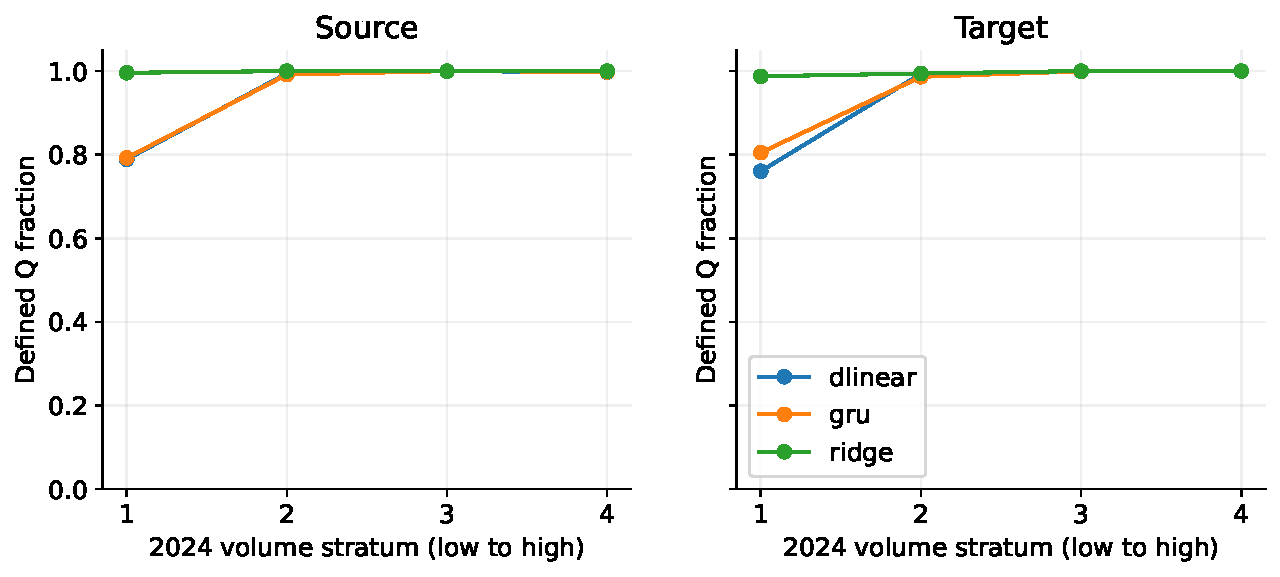
\includegraphics[width=.9\textwidth]{replication_denominators.pdf}
\caption{Defined h1 source-calendar Shapley score fractions by 2024 volume stratum, combining seeds and both operators. Undefined response denominators remain in the audit. More queried timestamps do not guarantee informative rankings for every institution.}\label{fig:denom}
\end{figure*}

A concrete example separates numerical validity from accuracy (Fig.~\ref{fig:local}): institution 132 at its earliest selected 2025 origin, 15 April 00:00 UTC, frozen GRU seed 42. This metadata-based rule does not choose forecast success. Predicted h1 is 0.322 GB versus observed 0.00665 GB; h6 is 1.479 versus 0.184 GB. Both reference-specific local IG allocations pass at 64 nodes, yet the forecast is overestimated. The attribution pattern changes with reference because the prediction contrast changes.

\begin{figure*}[t]\centering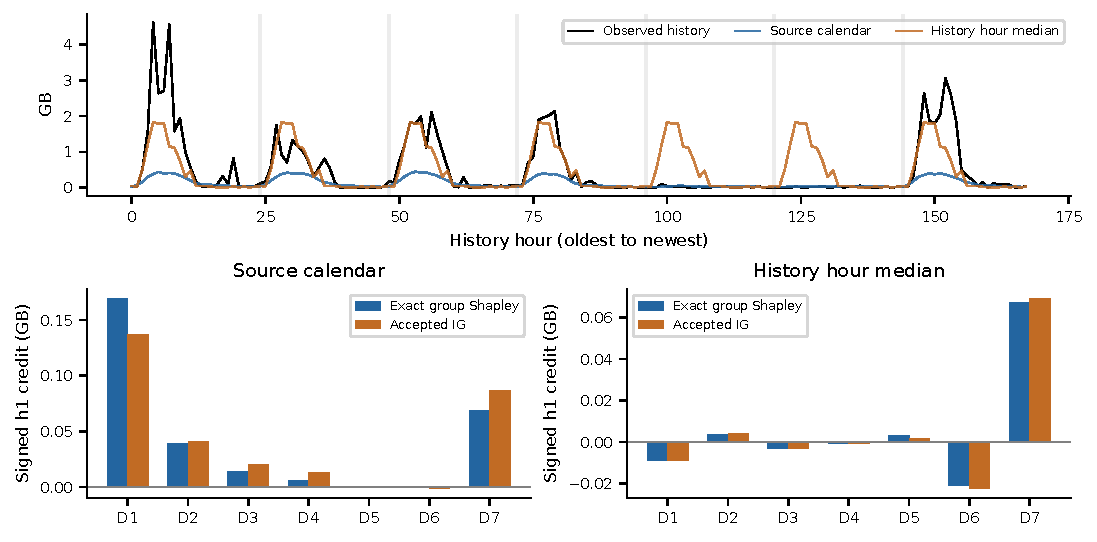
\includegraphics[width=\textwidth]{paper_local_case.pdf}
\caption{Metadata-selected original-cohort example. Top: history and references. Bottom: signed h1 daily Shapley/accepted-IG allocations, oldest day first. Numerical acceptance and exact allocation do not imply forecast success or causal demand attribution.}\label{fig:local}
\end{figure*}

\section{Discussion, Reproducibility and Limitations}
The expanded evidence supports a bounded conclusion: the fixed primary test does not detect systematic transfer degradation, while neither a zero-containing interval nor more queries proves equivalence or reliability for excluded regimes. Reference choice, numerical screening and oracle-gap availability change what is summarized. The original reference-specific secondary pattern does not recur in the larger cohort; selecting it as the headline would misrepresent the full evidence.

All institutions share one ISP. Source anchors and trained models also overlap across cohorts; we neither pool them as independent replications nor identify a causal effect of institutional novelty. Complete-history selection may favor regular regimes and excludes interrupted observations. Missing periods, common academic calendars and only two years limit bootstrap coverage; 14-day blocks cannot guarantee independence. Intervals are nominal and conditional on valid complete cells. Matching does not remove residual institutional differences.

The operators are controlled stress tests, not validated conditional traffic draws. They can reward undesirable model sensitivity. Seven daily groups suppress intra-day detail; IG uses finite quadrature and four sampled main origins. The model/explainer set omits foundation forecasters and specialized methods such as TimeSAE. Secondary comparisons have no multiplicity correction. An independent network, conditional replacement validation and specialized baselines remain useful external tests.

The artifact includes frozen protocols, selection/matching, code/data/model hashes, 80 unique selected series across the projects, checkpoints, predictions, exclusions, notebooks and complete analysis tables. New-cohort manifests hash 100 inputs. Audits recompute saved forecast metrics, re-query predictions and labels, check Shapley by permutations and independently reconstruct main/dense points; reused main/dense rows agree exactly. The original full notebook rerun reproduces all neural parameter tensors and the primary result. Supplementary figures preserve training/coverage, numerical breakdowns and exploratory agreement diagnostics.

On a four-thread Apple M5 CPU, the original full rerun takes 529.5 seconds, including 324.3 seconds of training. New main/dense XAI takes 18.7/16.3 minutes with no refitting. Compact models, sampled epochs and cached 128-coalition response games explain the workload. Runtime and record count do not establish validity or additional independent institutions.

\section{Conclusion}
An institution-disjoint forecasting benchmark benefits from separate accuracy, numerical and ranking evidence. Across an original target cohort and a separately frozen larger cohort, primary intervals do not establish degradation or equivalence. Undefined ranking games and low-volume forecast failures constrain the apparent informative-case result. The conference contribution is a reproducible empirical attribution-reliability audit with explicit references, controlled operators, effective denominators and bounded within-network conclusions.

\IEEEtriggeratref{15}
\bibliographystyle{IEEEtran}
\begingroup
\interlinepenalty=10000
\bibliography{references}
\endgroup
\end{document}
